\chapter{ミリ波観測手法}
\label{ch:mm_obs}

\ref{ch:mm_obs}章では我々が用いるミリ波分光を用いた観測手法について述べる。
まず\ref{sec:mm_obs}節では観測手法について、また観測された電波強度に対して黒体を用いたキャリブレーション手法と、分子スペクトルを抽出するために行う電波強度の補正に用いる周波数スイッチングと、光学的厚みの測定について述べていく。
次にそれぞれの観測場所で用いられた分光計において、\ref{sec:mm_tromsoe}節でノルウェー・トロムソ(Troms\o , Norway)、\ref{sec:mm_syowa}節で南極・昭和基地(Syowa, Antarctic)について述べていく。

\section{観測手法}
\label{sec:mm_obs}

最初にミリ波分光を用いた観測手法について述べる。
私たちのグループでは、観測の手法としてミリ波電波分光法による地上観測を用いて大気分子を観測している~\cite{mizuno2002millimeter}。
その模式図を図\ref{fig:spectrometer_schema}に示す。
\begin{figure}[htbp]
    \centering
    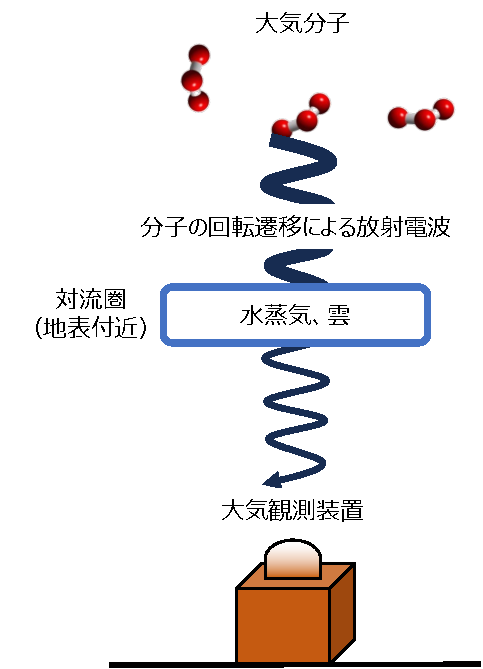
\includegraphics{master_thesis_contents/master_thesis_fig/spectrometer_schema.pdf}
    \caption{ミリ波電波分光法による地上観測の模式図}
    \label{fig:spectrometer_schema}
\end{figure}
ミリ波電波分光法では、観測対象の大気分子の回転遷移によって放射されるミリ波帯電波を受信し分光することで、電波放射スペクトルを観測している。
しかし、図\ref{fig:spectrometer_schema}に示す通りに電波を地上観測する上で下層大気の水蒸気や雲の影響を考慮する必要があり、そのために光学的厚みを計算する。
およそ5分間隔の積分時間で大気分子スペクトルを観測し、その5分の間隔の間に光学的厚みを測定している。
% 間隔時間はトロムソと昭和で一緒?
光学的厚みの測定方法の詳細は後述する。
ミリ波大気観測装置の概略図を図\ref{fig:mm_component}に示し、南極・昭和基地にて実際に設置されたミリ波分光計の様子を図\ref{fig:mmobs_spectrometer_syowa}に示す。
図\ref{fig:spectrometer_schema}に示すように観測装置は主に4つの部分に分かれている。
\begin{figure}[htbp]
    \centering
    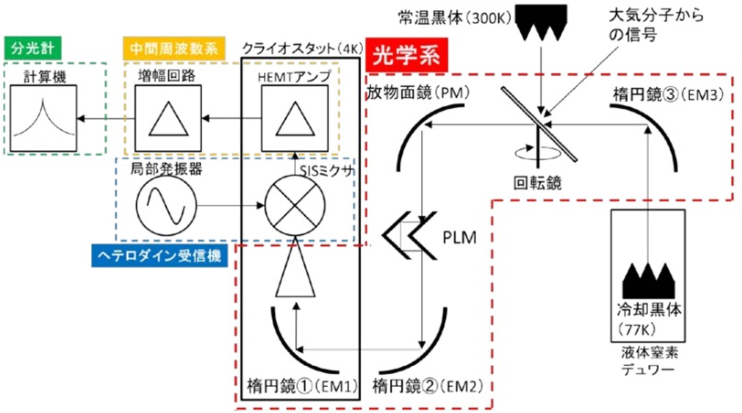
\includegraphics[width=\linewidth]{master_thesis_contents/master_thesis_fig/mm_component.pdf}
    \caption{ミリ波大気観測装置の概略図(~\cite{ito2017master}より引用)}
    % \caption{$\scriptstyle \mbox{ミリ波大気観測装置の概略図}\atop \scriptstyle \mbox{text}(~\cite{ito2017master}より引用$}
    \label{fig:mm_component}
\end{figure}
\begin{figure}[htbp]
    \centering
    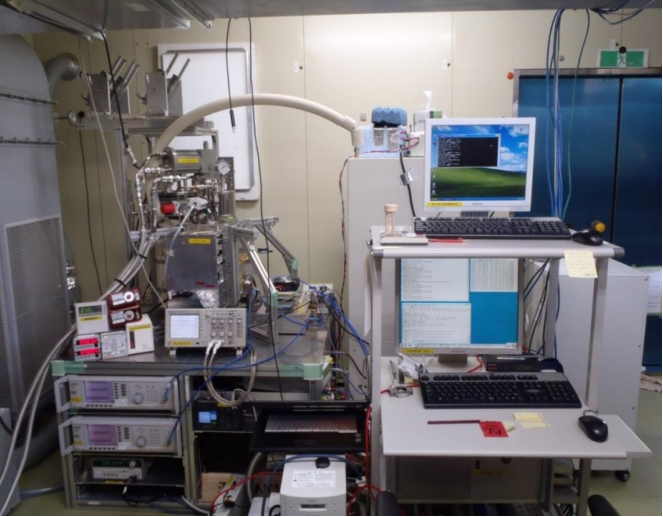
\includegraphics[width=\linewidth]{master_thesis_contents/master_thesis_fig/mmobs_spectrometer_syowa.pdf}
    \caption{南極の昭和基地に設置された観測装置(~\cite{uemura2014master}より引用)}
    \label{fig:mmobs_spectrometer_syowa}
\end{figure}
\begin{enumerate}
    \item 光学系 \mbox{} \\
        大気分子からの電波と、電波強度から黒体温度に変換する(詳細は後述)際に用いる常温黒体と冷却黒体からの電波を受信機内部まで集光し伝送する。
        また、回転鏡を用いることにより、大気観測における観測天頂角を変えることで光学的厚みの測定(詳細は後述)を行っている
    \item ヘテロダイン受信機 \mbox{} \\
        大気分子からの信号を局部発振器からの信号をミクサで混合している。
        大気分子からの電波は微弱であり、信号処理に適切なレベルまで増幅しなければならない。
        しかし、本研究で扱う電波の周波数(数百$GHz$程度)を直接増幅できる増幅器は実用レベルでは存在しない。
        そこで、観測装置で受信した信号をいったん低い周波数に下げることにより増幅する方法をとっている。
    \item 中間周波数系 \mbox{} \\
        低周波に変換された信号を分光計に適切な周波数にさらに変換し、分光計に必要なレベルまで増幅する。
    \item 分光計 \mbox{} \\
        デジタル高速フーリエ変換により分光処理を行い、大気分子のスペクトルを得る。
        入力信号を直接A/D変換して時系列データとして読み込み、それを高速フーリエ変換することにより周波数スペクトルを得ている。
        本研究で用いるデータを得るために用いられた分光計は16348チャンネルの周波数スペクトルデータを出力する~\cite{ito2017master}。
        % 昭和基地の場合のチャンネル数は?引用元をみないといけない
\end{enumerate}
ミリ波電波分光法による地上観測による利点は、太陽光などの背景光源を必要とせず昼夜モニタリングが可能となることである。
昼夜だけでなく白夜や極夜がある極地においても、その影響を受けずに連続観測することができる。
以上より、連続的・長期的に観測を行うことが可能で、自然起源や人為起源による長期的変動や短期的変動を観測することが可能であり、これが我々の研究グループでミリ波電波分光法による地上観測を用いる理由である。


次に、観測された電波強度に対して行う黒体を用いたキャリブレーション手法について述べる。
本研究では、大気分子からの電波強度は、それと同等のエネルギーを放射する黒体の温度に換算して表す。ミリ波領域(周波数$30-300\, \mathrm{GHz}$)においては図\ref{fig:planck}よりRayleigh-Jeans近似が成り立つので、Planckの放射式は以下のように表すことができる。
\begin{gather}
    I_\nu(T)
    = \frac{2h\nu^3}{c^2} \cdot \cfrac{1}{\exp\left(\cfrac{h\nu}{kT}-1\right)}
    \approx \frac{2h\nu^3}{c^2} \cdot \left(\frac{h\nu}{kT}\right)^{-1}
    = \frac{2\nu^2}{c^2}kT \\
    I_\nu(T):電波強度、c:光速、k:Boltzmann定数、h:Planck定数、\nu:周波数、T:黒体温度 \notag
    \label{eq:planck}
\end{gather}
\begin{figure}[htbp]
    \centering
    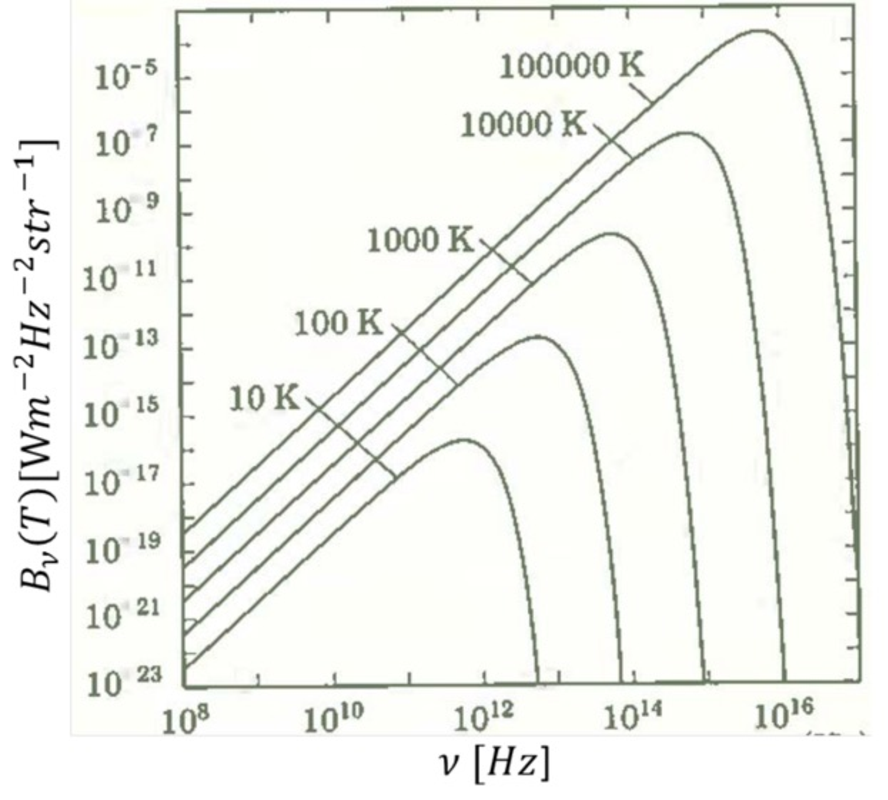
\includegraphics[width=\linewidth]{master_thesis_contents/master_thesis_fig/planck.pdf}
    \caption{Planckの放射式(~\cite{ito2017master}より引用)}
    \label{fig:planck}
\end{figure}
このように黒体温度と電波強度は比例の関係になり、大気分子からの電波強度を黒体の温度に換算することが可能である。
具体的には常温黒体(典型値として$300\, \mathrm{K}$)と液体窒素で冷却された黒体($77\, \mathrm{K}$)からの電波放射を受信機に入れることにより電波強度と黒体温度を対応させる。
\begin{figure}[htbp]
    \centering
    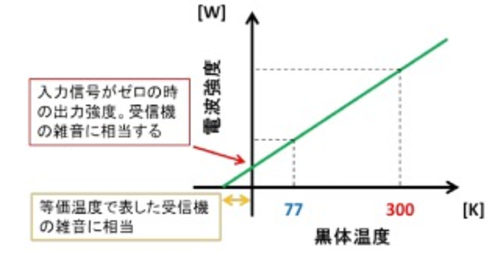
\includegraphics[width=\linewidth]{master_thesis_contents/master_thesis_fig/calibration.pdf}
    \caption{電波強度のキャリブレーションの様子(~\cite{ito2017master}より引用)}
    \label{fig:calibration}
\end{figure}
図\ref{fig:calibration}に示す直線が電波強度と黒体温度の対応を示している。
また直線の$y$切片の値は受信機雑音を示し、$x$切片の値の絶対値は受信機雑音を黒体温度で表した値となる。


次に、電波強度の補正に用いる光学的厚みについて述べる。
また、図\ref{fig:spectrometer_schema}に示す通りに、成層圏よりも高い高度を分子スペクトルを地上で観測する際には、下層大気(主に対流圏)を通過してきた電波を観測することになる。
そのため、下層大気に含まれる水蒸気や雲の放射や吸収の影響を考慮に入れるため、光学的厚みという概念を導入する。


光学的厚みがどのように電波強度に影響するかを述べる。
図\ref{fig:depth_dx}のように、厚さ$dx$の大気層があり、図の左から強度$T$の電波が入射したときを考える。
大気層で吸収および放射の影響を受けて、図の右に出てくる電波強度は$T+dT$で表される。
\begin{figure}[htbp]
    \centering
    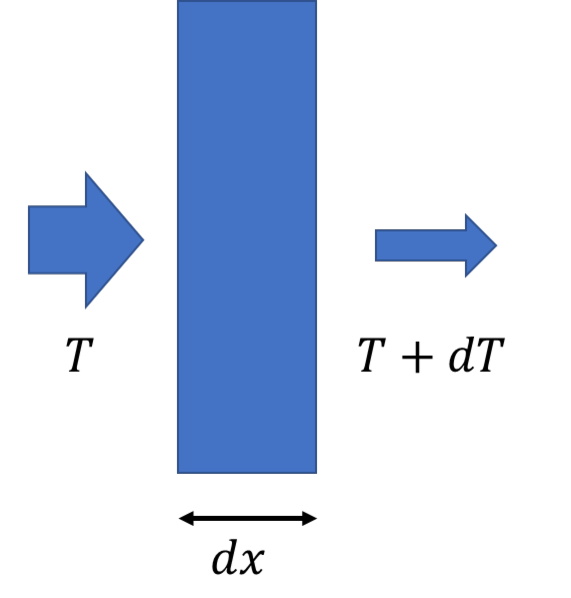
\includegraphics[width=\linewidth]{master_thesis_contents/master_thesis_fig/depth_dx.pdf}
    \caption{厚さ$dx$の大気層を通過する電波強度の模式図}
    \label{fig:depth_dx}
\end{figure}
このとき、吸収と自己放射を表す式は、$\kappa$を吸収係数、$j$を放射係数とすると
\begin{equation}
    dT = -\kappa T dx + j dx
    \label{eq:absorption_selfemission_1}
\end{equation}
となる。
次に光学的厚み(一般的に$\tau$で表す)を導入する。$\tau$は、
\begin{equation}
    \tau = \int_{0}^{x} \kappa dx' + j dx
\end{equation}
もしくは
\begin{equation}
    d\tau = \kappa dx
\end{equation}
と表され、これを用いて式\refeq{eq:absorption_selfemission_1}を書き換えると
\begin{equation}
    \frac{dT}{d\tau} = -T + \frac{j}{\kappa}
    \label{eq:absorption_selfemission_4}
\end{equation}
となる。
次に、式\refeq{eq:absorption_selfemission_4}の第2項において、熱平衡状態ではキルヒホッフの法則より
\begin{gather}
    \frac{j}{\kappa}
    = \frac{2h\nu^3}{c^2} \cdot \cfrac{1}{\exp\left(\cfrac{h\nu}{kT}-1\right)}
    \equiv I_\nu
    = T_\mathrm{sky} \\
    % I_\nu :電波強度、T_{sky}:大気からの熱放射、c:光速、k:Boltzmann定数 \notag \\
    % h:Planck定数、\nu :周波数、T:黒体温度 \notag
    T_\mathrm{sky}:大気からの熱放射 \notag
    \label{eq:absorption_selfemission_5}
\end{gather}
が成り立つ。
これを利用して式\refeq{eq:absorption_selfemission_5}より式\refeq{eq:absorption_selfemission_4}の解を求めると、
\begin{gather}
    T = T_0\exp\left(-\tau\right) + T_\mathrm{sky}\left(1-\exp\left(-\tau\right)\right) + T_\mathrm{sys} \\
    T_0 :大気分子からの電波強度、T_\mathrm{sky}:受信機雑音 \notag
    \label{eq:absorption_selfemission_6}
\end{gather}
となる。
これは、第1項が下層大気による電波吸収を考慮した(より上層にある)観測対象の分子からの電波強度、第2項は下層大気の熱放射を表している。
実際の観測で得られるスペクトルデータとしては第1項が図\ref{fig:spectum_thermalnoise}における橙色の成分、第2項が青色の成分に対応する(実際には青色の成分に受信機雑音も含まれるが、その詳細はこの後述べる)。
\begin{figure}[htbp]
    \centering
    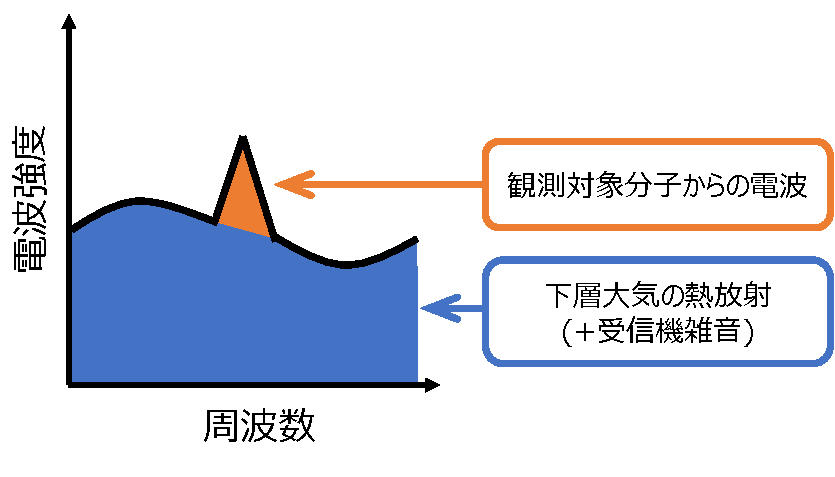
\includegraphics[width=\linewidth]{master_thesis_contents/master_thesis_fig/spectum_thermalnoise.pdf}
    \caption{スペクトルデータの強度を決める要素}
    \label{fig:spectum_thermalnoise}
\end{figure}
式\refeq{eq:absorption_selfemission_6}の左辺$T$が観測データから直接的に得られる値であるが、我々が知りたい値は、もともとの放射強度である$T_0$であるので、$T_0$を知るためには光学的厚みによる補正が必要となるわけである。(光学的厚みの測定方法の詳細は後述する。)


観測対象の分子スペクトルを得るために、大気の熱放射と観測装置の受信機からのノイズによるオフセット成分を除去する必要があり、周波数スイッチング(以後FRSWとする)という手法を用いる(図\ref{fig:frsw_schema})。
\begin{figure}[htbp]
    \centering
    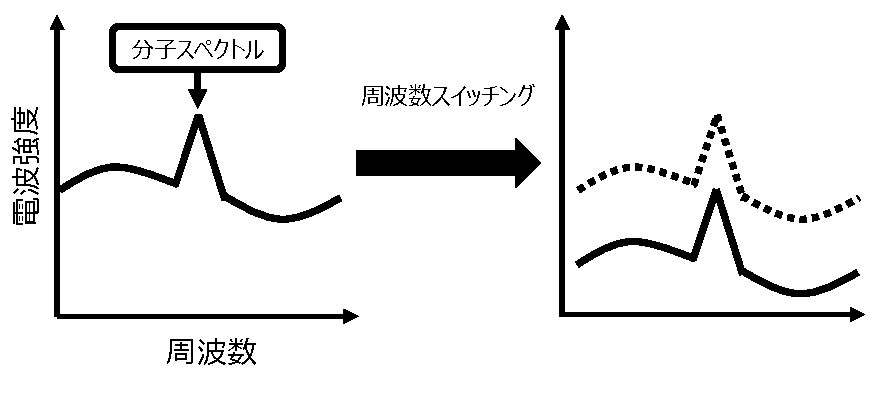
\includegraphics[width=\linewidth]{master_thesis_contents/master_thesis_fig/frsw_schema.pdf}
    \caption{周波数スイッチング(FRSW)の模式図}
    \label{fig:frsw_schema}
\end{figure}
FRSWによるオフセット成分の除去はおおまかなものであり、本研究では弱いスペクトルを検出する必要があるため、さらに細かくオフセット成分を補正する必要があるが、その詳細は\ref{sec:correction_baselinefitting}節で述べる。
本研究では、FRSWに加えて周波数折返し処理という解析方法を用いることで、オフセット成分を除去するとともに、スペクトルデータの信号対雑音比(S/N比)を向上させている。
\begin{figure}[htbp]
    \centering
    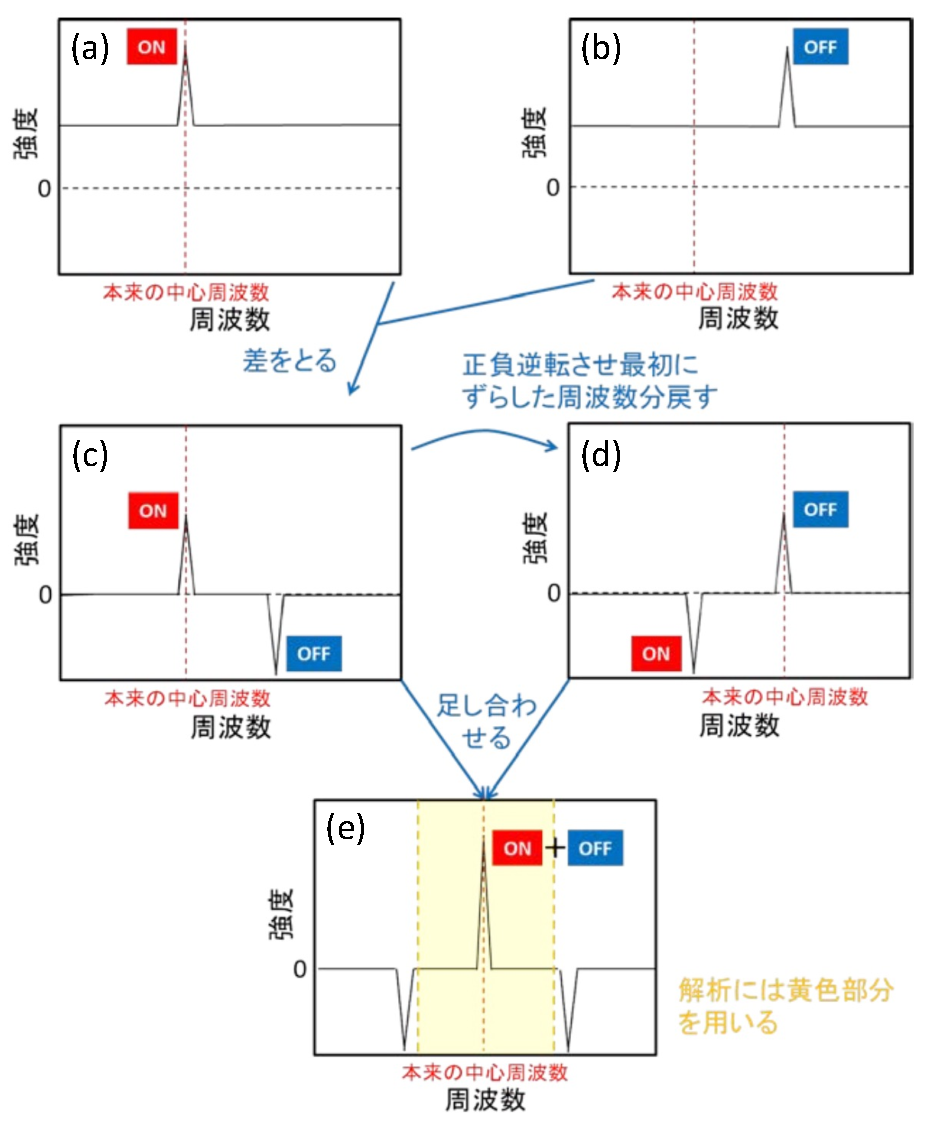
\includegraphics[width=\linewidth]{master_thesis_contents/master_thesis_fig/frsw_process.pdf}
    \caption{周波数スイッチングと周波数折り返し処理の概要(\cite{ito2017master}より引用)}
    \label{fig:frsw_process}
\end{figure}
まず、元となる最初に取得されたデータを図\ref{fig:frsw_process}(a)に示す。
次に、本来の局部発振器周波数から$\Delta f$だけ周波数をずらしたデータを取得する(図\ref{fig:frsw_process}(b))。
解析では、まず(a)から(b)を差し引いたデータを作成する(図\ref{fig:frsw_process}(c))。
これにより、(a)から(b)に共通に乗っていたオフセット成分が差し引かれる。
さらに(c)を上下反転して、ずらした周波数$\Delta f$を戻した(d)を作成する。
この(d)と(c)のデータを足し合わせて2で割る処理をする(周波数折り返し処理)。
(a)と(b)で取得された輝線スペクトルのデータは独立なものなので、この処理をすることによって、S/N比が$\sqrt{2}$倍向上する(図\ref{fig:frsw_process}(e))。
最終的に得られる分子スペクトルは図\ref{fig:frsw_process}(e)中の黄色で囲まれたところのみを使う。


次に、光学的厚みをどのように測定するかについて述べる。
光学的厚みの測定は図\ref{fig:opticaldepth_measurement}のように観測の間に行われており、トロムソの観測装置ではおよそ5分おきに測定されている。
% 昭和基地も同じなのか?
% 図を改良する必要あり
\begin{figure}[htbp]
    \centering
    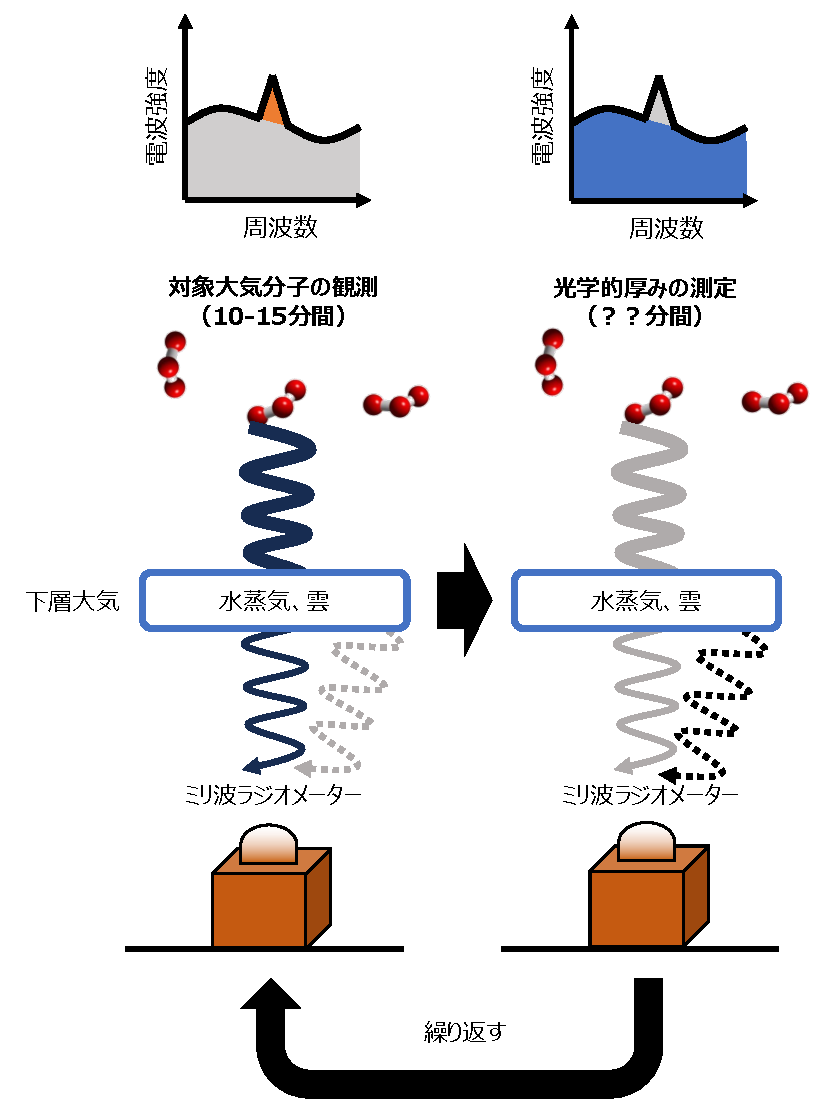
\includegraphics[width=\linewidth]{master_thesis_contents/master_thesis_fig/opticaldepth_measurement.pdf}
    \caption{ミリ波観測と光学的厚み$(\tau)$の測定の流れ}
    \label{fig:opticaldepth_measurement}
\end{figure}
測定された光学的厚みは直前に観測された電波強度のデータの補正に用いられる。
光学的厚みの測定についてはSky tippingと呼ばれる手法が用いられる。
まず関係式として、
\begin{gather}
    \begin{cases}
        T_z = T_\mathrm{sky}\{ 1-\exp (-\tau \sec z) \} + T_\mathrm{sys} \\
        T_\mathrm{obs\_ hot} = T_\mathrm{hot} + T_\mathrm{sys}
    \end{cases}
    \label{eq:opticaldepth_measurement} \\ \notag
    z :観測する角度の天頂角 \\ \notag
    T_\mathrm{z} :天頂角zでの分子スペクトルを含まない周波数の信号強度 \\ \notag
    % T_{sky} :大気からの熱放射、T_{sys} :観測装置の自己雑音温度 \\ \notag
    T_\mathrm{obs\_ hot} :常温黒体を見たときの輝度温度 \\ \notag
\end{gather}
ここで、$T_\mathrm{sky} = T_\mathrm{hot}$と仮定し式\refeq{eq:opticaldepth_measurement}の2式の差をとって両辺対数をとると
\begin{equation}
    \ln \left( T_{obs\_ hot} - T_z \right)  = \ln T_{obs\_ hot} - \tau \sec z
    % \ln \( T_{obs\_ hot} - T_z \) = \ln T_{obs\_ hot} - \tau \sec z
\end{equation}
この式は$y=ax$のような一次関数になっているため、左辺$\ln \left( T_\mathrm{obs\_ hot} - T_z \right)$を縦軸、$\sec z$を横軸としたプロットを作成すると図\ref{fig:opticaldepth_slope_tau}のようになることがわかる(プロットデータは観測装置の回転鏡により$z$の値を変えている)。
これらのプロットに対して一次の近似直線を引いたとき、その直線の傾きが光学的厚みに負の符号をつけたものと対応する。
以上より、光学的厚みを観測的に求めることができる。
\begin{figure}[htbp]
    \centering
    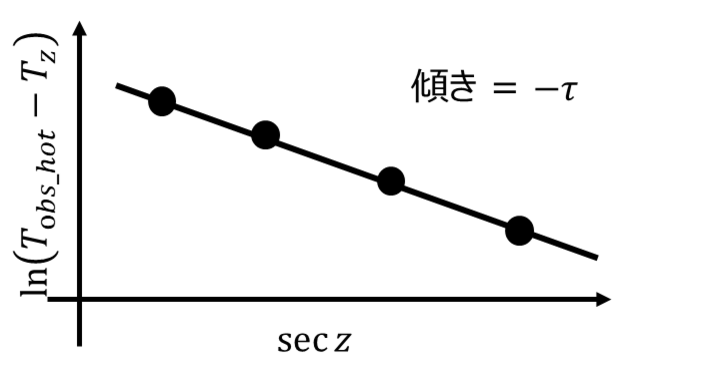
\includegraphics[width=\linewidth]{master_thesis_contents/master_thesis_fig/opticaldepth_slope_tau.pdf}
    \caption{光学的厚み$\tau$を求めるためのプロットデータ}
    \label{fig:opticaldepth_slope_tau}
\end{figure}
トロムソの観測装置で実際に測定している$\sec z$の値は表\ref{tb:secz_zdeg}のようになっている。
ここでは、それに対応した天頂角$z$と仰角の値も示す。
\begin{table}[htbp]
    \centering
    \caption{$\sec z$と天頂角$z\ [ \deg ]$と仰角$[ \deg ]$との対応}
    \label{tb:secz_zdeg}
    \setlength{\belowcaptionskip}{5mm}
    \begin{tabular}{ccc}
    \hline
    $\sec z$ & 天頂角 $z\ [ \deg ]$ & 仰角$[ \deg ]$ \\ \hline
    1.46     & 47                & 43           \\ \hline
    1.83     & 57                & 33           \\ \hline
    2.28     & 64                & 26           \\ \hline
    2.79     & 69                & 21           \\ \hline
    \end{tabular}
\end{table}
次の\ref{sec:mm_tromsoe}節と\ref{sec:mm_syowa}節では、それぞれ観測を立ち上げた時期と設置されてきた分光計の概要を述べる。トロムソと昭和基地で設置された分光計の仕様を表\ref{tb:spectrometer_spec}に示す。
% Single frequencyは「単周波数分光計」と訳せばいいのか?
\begin{table}[htbp]
    \centering
    \caption{トロムソ(1段目)と昭和基地(2段目)で設置された分光計の仕様}
    \label{tb:spectrometer_spec}
    \setlength{\belowcaptionskip}{5mm}
    \resizebox{\columnwidth}{!}{%
    \begin{tabular}{ccccc}
    \hline
    &
        期間 &
        FrontEnd &
        BackEnd &
        観測対象の分子 \\ \hline
    単周波数分光計 &
        \begin{tabular}[c]{@{}c@{}}2012年1月 –\\ 2020年8月\end{tabular} &
        \begin{tabular}[c]{@{}c@{}}1 Double sideband\\ PCTJ  SIS mixer\end{tabular} &
        \begin{tabular}[c]{@{}c@{}}FFT 分光計\\ 帯域 $\sim$1 GHz\\ 分解能 $\sim$61 kHz\end{tabular} &
        \begin{tabular}[c]{@{}c@{}}\ce{NO}, \ce{O3} \\ (分子同時観測不可能)\end{tabular} \\ \hline
    % Multi-freq. Phase 1 &
    %     \begin{tabular}[c]{@{}c@{}}2020年11月 – \\ 2021年2月\end{tabular} &
    %     \begin{tabular}[c]{@{}c@{}}2 Single sideband\\ PCTJ SIS mixers\end{tabular} &
    %     \begin{tabular}[c]{@{}c@{}}FFT 分光計\\ 帯域 $\sim$1GHz\\ 分解能 $\sim$61 kHz\end{tabular} &
    %     \begin{tabular}[c]{@{}c@{}}\ce{NO}, \ce{O3}, \ce{CO}, \ce{HO2} \\ (分子同時観測可能)\end{tabular} \\ \hline
    % Multi-freq. Phase 2 &
    %     \begin{tabular}[c]{@{}c@{}}2021年3月 –\\ 2022年1月\end{tabular} &
    %     \begin{tabular}[c]{@{}c@{}}1 Single sideband\\ PCTJ SIS mixers\end{tabular} &
    %     \begin{tabular}[c]{@{}c@{}}FFT 分光計\\ 帯域 $\sim$2 GHz\\ 分解能 $\sim$61 kHz\end{tabular} &
    %     \begin{tabular}[c]{@{}c@{}}\ce{NO}, \ce{O3}, \ce{HO2} \\ (分子同時観測可能)\\ (due to oscillator damage)\end{tabular} \\ \hline
    多周波数分光計 &
    % 多周波数分光計 Phase 3 &
        2022年7月 – &
        \begin{tabular}[c]{@{}c@{}}2 Single sideband\\ series-array SIS mixers\end{tabular} &
        \begin{tabular}[c]{@{}c@{}}FFT 分光計\\ 帯域 $\sim$2.5 GHz\\ 分解能 $\sim$76 kHz\end{tabular} &
        \begin{tabular}[c]{@{}c@{}}\ce{NO}, \ce{O3}, \ce{CO}, \ce{NO2}, \ce{HO2}\\ (分子同時観測可能)\end{tabular} \\ \hline
    \end{tabular}
    }
\end{table}
% \afterpage{\clearpage}
\clearpage

\section{Troms\o , Norway(69.35\textdegree N, 19.14\textdegree E)}
\label{sec:mm_tromsoe}
% \begin{itemize}
%     \item 観測立ち上げが行われた背景
%     \item いつ観測立ち上げが行われたか
%     \item 分光計の概要(とくに帯域について)
% \end{itemize}
\ref{sec:intro_privious}節で述べた、ミリ波分光観測において夏に短期変動の観測ができないという課題を解決するためには、北極域において同様の観測を実施することにより、両極域で\ce{NO}の同時モニタリングをすることが必要である。
両極において日照時間の長さは真逆の関係になっており、一方の極が夏期ならもう一方の極は冬期になる。
したがって、光化学反応の影響を強く受ける夏期ではわからない場合に、同時期のもう一方の冬期の極でデータを取得して比較することで、高エネルギー電子の降り込み(EPP: Energetic Electron Precipitation)による短期間変動を定量的に切り分けることができると考えた。
そこで我々は、北極域での観測拠点としてノルウェーのトロムソにあるEISCAT(European Incoherent Scatter)レーダー観測所に、2015年から2016年にかけて新たな観測装置を設置した~\cite{ito2017master}。
トロムソは南極の昭和基地とおよそ地磁気緯度が同じであるため、大きなEPPが起きると同時に影響を受けると期待できる。
観測所を利用することで、観測立ち上げのために新たにインフラを整備する必要がないという利点があるほか、EISCATレーダーの観測によって得られる電子密度などのデータを用いて、電子降り込みに関する情報と比較することができるということも重要である。
トロムソはミリ波地上観測にとってははじめての観測地であるため、周囲の電波環境や新たな観測装置の特性は明らかではなく、実際にどのような質のデータが取れるのかということの確認が必要である。
そのため、取得データを科学的研究に最大限に活用するためには、まずはデータの傾向を精査する必要がある。
そして、その傾向を把握した上で、データのスクリーニング(特定の条件を設定し、全体のデータから解析に用いることができるデータのみを選別)をする必要がある(詳細は\ref{sec:screening_opticaldepth}節と\ref{sec:screening_spectralnoise}節にて述べる)。
今回は2018年12月26日 - 2019年3月10日の期間に行われたテスト観測データを用いた。


\section{Syowa, Antarctic(69.00\textdegree S, 39.85\textdegree E)}
\label{sec:mm_syowa}
% \begin{itemize}
%     \item いつ観測立ち上げが行われたか
%     \item 過去の分光計の概要(とくに帯域について)
%     \item 多周波数分光計の設置
% \end{itemize}
南極・昭和基地では2011年に観測装置が立ち上げられ、現在まで観測が続けられている。
% 立ち上げが2011年?観測開始が2012年?
% 分光計は4つすべて用いられた?
今回は2023年3月22日 - 2023年3月30日の観測データを用いた。
昭和基地では\ce{O3}と\ce{NO}の同時観測を目指すため、多周波数分光計が設置されている。
今回用いた分光計は2022年7月より定常観測を行っており、分光帯域は従来の分光計と比較して$1\, \mathrm{GHz}$から$2.5\, \mathrm{GHz}$まで広がった(表\ref{tb:spectrometer_spec})。
帯域が広がったことにより観測できる\ce{NO}の輝線スペクトルの本数を増やすことができた。トロムソに設置されている分光計では2本の輝線スペクトルが観測できたが、昭和基地では6本の輝線スペクトルを観測することができた。
現在観測できる\ce{NO}の輝線スペクトル例を図\ref{fig:NO_spectr}に示す。
黒枠が南極・昭和基地で観測できる6本の\ce{NO}スペクトルを表し、赤枠がトロムソで観測できる2本の輝線スペクトルを表す。
観測しているそれぞれの輝線スペクトルの周波数と遷移については、表\ref{tb:no_spectr_freq}に示す。
なお、\ce{NO}スペクトルの周波数は、NASAが提供しているNASA JPL Catalog\footnote{\url{https://spec.jpl.nasa.gov/ftp/pub/catalog/catform.html}}より調べた。
線スペクトル強度係数は柱密度の導出に用いるパラメーターである。(詳細は\ref{sec:derive_columndensity}節)。
\begin{figure}[htbp]
    \centering
    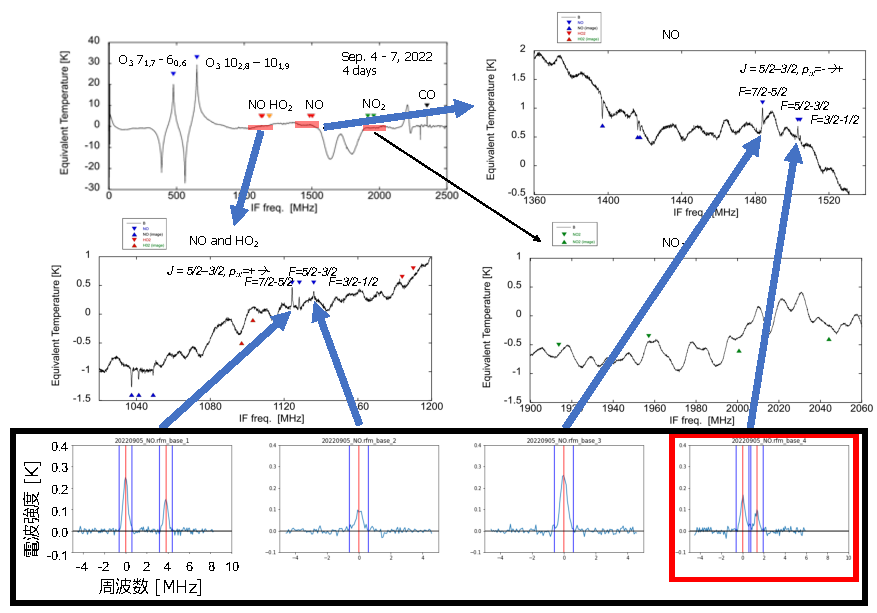
\includegraphics[width=\linewidth]{master_thesis_contents/master_thesis_fig/NO_spectr.pdf}
    % \caption{$\scriptstyle \mbox{昭和基地で現在観測できる6本の\ce{NO}輝線スペクトル} \scriptstyle
    % \mbox{(黒枠。赤枠はトロムソで観測できる2本の輝線スペクトル)}$}
    \caption{昭和基地で現在観測できる6本の\ce{NO}輝線スペクトル}
    % \caption{\protect 昭和基地で現在観測できる6本の\ce{NO}輝線スペクトル \linebreak
    % (黒枠。赤枠はトロムソで観測できる2本の輝線スペクトル)}
    \label{fig:NO_spectr}
\end{figure}
\begin{table}[htbp]
    \centering
    \caption{トロムソと昭和基地で観測される6本の\ce{NO}の輝線スペクトル}
    \label{tb:no_spectr_freq}
    \resizebox{\textwidth}{!}{%
    \begin{tabular}{cccccccc}
    \hline
    周波数 & \multicolumn{2}{c}{観測可能} & $J$ & $P_{\mathrm{ul}}$ & $F$ & IF 周波数  & 線スペクトル強度係数 $A$ \\
    $[\mathrm{GHz}]$ & Troms\o & Syowa &  &  &  & $[\mathrm{MHz}]$ & $[\mathrm{K^{-2}} \mathrm{MHz^{-1}} \mathrm{cm^{-2}}]$ \\ \hline
    $250.436848$ &  & $\circ$ & $5/2 - 3/2$ & \ce{+ -> -} & $7/2 - 5/2$ & $1124.3$ & $4.00\times 10^{13}$ \\ \hline
    $250.440659$ &  & $\circ$ & $5/2 - 3/2$ & \ce{+ -> -} & $5/2 - 3/2$ & $1128.2$ & $6.35\times 10^{13}$ \\ \hline
    $250.448530$ &  & $\circ$ & $5/2 - 3/2$ & \ce{+ -> -} & $3/2 - 1/2$ & $1136.0$ & $1.07\times 10^{14}$ \\ \hline
    $250.796436$ &  & $\circ$ & $5/2 - 3/2$ & \ce{- -> +} & $7/2 - 5/2$ & $1483.9$ & $3.99\times 10^{13}$ \\ \hline
    $250.815954$ & $\circ$ & $\circ$ & $5/2 - 3/2$ & \ce{- -> +} & $5/2 - 3/2$ & $1503.1$ & $6.33\times 10^{13}$ \\ \hline
    $250.816954$ & $\circ$ & $\circ$ & $5/2 - 3/2$ & \ce{- -> +} & $3/2 - 1/2$ & $1504.5$ & $1.06\times 10^{14}$ \\ \hline
    \end{tabular}%
    }
\end{table}

\ce{O3}の輝線スペクトルと比較すると\ce{NO}の輝線スペクトルはとても微弱である。
そのため、どのデータが解析に用いることができるかスクリーニングを行い、電波強度の補正を行うことが重要となってくる。
詳細は\ref{ch:mm_analysis}章で述べていく。
